\begin{enumerate}[label=\thesection.\arabic*.,ref=\thesection.\theenumi]
\numberwithin{equation}{enumi}

\item
Match the transfer functions of the second-order systems with the nature of the systems given below

\underline{Transfer functions}
\hspace{20mm}
\underline{Systems}
\vspace{5mm}
\newline P &:$\frac{15}{{s^2+5s+15}}$
\hspace{20mm}
1:Overdamped
\vspace{2mm}
\newline Q &:$\frac{25}{{s^2+10s+25}}$
\hspace{20mm}
2:critically damped
\vspace{2mm}
\newline R &:$\frac{35}{{s^2+18s+35}}
\hspace{20mm}
3:Underdamped


\begin{align}
  (A)P-1,Q-2,R-3
\end{align}
\begin{align}
(B)P-2,Q-1,R-3
\end{align}
\begin{align}
 (C)P-3,Q-2,R-1
\end{align}
\begin{align}
 (D)P-3,Q-1,R-2
\end{align}
\solution The standard transfer function is H(s)=$\frac{\omega^2}{s^2+2\zeta\omega+\omega^2}\\
where \\"\omega"\hspace{2mm} is \hspace{2mm} natural \hspace{2mm} frequency \\ and "\zeta" \hspace{2mm}is\hspace{2mm} damping\hspace{2mm} factor\\
\vspace{2mm}

\newline then compare the given functions with this we get\\
\vspace{5mm}
 1. For Transfer function H(s)=$\frac{15}{s^2+5s+15}$, \\
\begin{align*}
     \omega^2 &= 15 \\ 2\zeta\omega &=5\\
    \text{then we get } \zeta &=$\sqrt{\frac{5}{12}} \textless 1
\end{align*}
2. For Transfer function H(s)=$\frac{25}{s^2+10s+25}$,\\
\begin{align*}
     \omega^2 &= 25 \\ 2\zeta\omega &=10\\
    \text{then we get } {\zeta} &= $\sqrt{\frac{5}{5}} = 1
\end{align*}
3. For Transfer function H(s)=$\frac{35}{s^2+18s+35}$,\\
\begin{align*}
    \omega^2 &= 35 \\ 2\zeta\omega &=18\\
    \text{then we get } {\zeta} &= $\sqrt{\frac{81}{35}} \textgreater 1
\end{align*}
The damping of a system can be described as being one of the following:
 

\newline \underline {Overdamped} &:
The system returns to equilibrium without oscillating.For this
\begin{align}
    \zeta \textgreater 1.
\end{align}


 
\begin{block}
\newline \underline{Critically damped}&:
The system returns to equilibrium as quickly as possible without oscillating.
\newline For this 
\begin{align}
    \zeta = 1
\end{align}

\end{block}

\begin{block}
\newline \underline{Underdamped}&:
The system oscillates(at reduced frequency compared to the undamped case) with the amplitude gradually decreasing to zero.
\newline For this 
\begin{align}
    0 \textless\zeta\textless1
\end{align}

\end{block}

\newline \underline{Undamped} &:
The system oscillates at its natural resonant frequency(\omega0).

\newline For this
\begin{align}
    \zeta &= 0
\end{align}

\newline \underline{Final Analysis}
\begin{itemize}
    \item As for P &: \zeta \textless 1
    \newline It is Underdamped system
    
    \item As for Q &: \zeta =1
     \newline It is critically damped system.
    
    \item As for R &: \zeta  \textgreater 1
    \newline It is an overdamped system.
\vspace{10mm}

   So,P-3,Q-2,R-1. Option (C) is correct.
\end{itemize}

%\usepackage{graphicx}
\begin{figure}
    \centering
    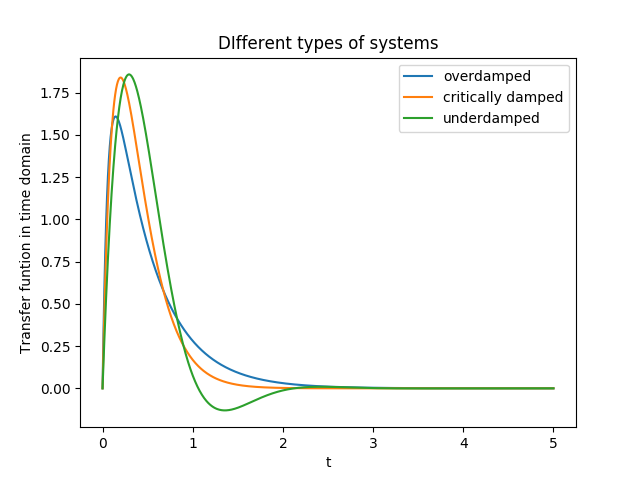
\includegraphics[width=0.7\linewidth]{Damping.png}
    \caption{Different systems based on \zeta}
    \label{fig:Graph}
\end{figure}




 











\end{enumerate}
